 \documentclass[12pt]{article}
\usepackage[T2A]{fontenc}
\usepackage[utf8]{inputenc}       

\usepackage[english]{babel}
\usepackage{amsmath,amsfonts,amsthm,amssymb,amsbsy,amstext,amscd,amsxtra,multicol}
\usepackage{verbatim}
\usepackage{tikz}
\usetikzlibrary{automata,positioning}
\usepackage{multicol}
\usepackage{graphicx}
\usepackage[colorlinks,urlcolor=blue]{hyperref}
\usepackage[stable]{footmisc}
\usepackage{ dsfont }
\usepackage{wrapfig}
\usepackage{xparse}
\usepackage{ifthen}
\usepackage{bm}
\usepackage{color}
 \usepackage{subfigure}
 
\usepackage{algorithm}
\usepackage{algpseudocode}

\usepackage{xcolor}
\usepackage{hyperref}
\definecolor{linkcolor}{HTML}{799B03} % цвет гиперссылок
\definecolor{urlcolor}{HTML}{799B03} % цвет гиперссылок
 
%\hypersetup{pdfstartview=FitH,  linkcolor=linkcolor,urlcolor=urlcolor, colorlinks=true}

\newtheorem{theorem}{Theorem}[section]
\newtheorem{lemma}{Lemma}[section]

\DeclareMathOperator{\sign}{sign}
\DeclareMathOperator{\grad}{grad}
\DeclareMathOperator{\intt}{int}
\DeclareMathOperator{\conv}{conv}
\begin{document}

\section{Данные}

В собранной коллекции имелось 100 пар текстов. Каждая пара состоит из написанного в спокойном состоянии и написанного в фрустрированном состоянии одним и тем же человеком текстов. Для каждого текста были вычислены одинаковые признаки (всего призноков 198), и для каждой пары была вычислена разница между текстами.

Перед нами ставится задача кластеризировать эту разницу, т.е. мы хотим сгруппировать людей по схожести шаблона изменения состояния со спокойного на фустрированное. Более того, добавим ограничение, что нас интересует качественная схожесть, а именно, мы будем считать, что если есть два человека, у которых некоторый признак при переходе состояния увеличивается, то значение этого признака не изменяется качественно. Это обуславливает далее описываемую предобработку данных.

Первый этап предобработки. Все признаки были отмасшатиборованы таким образом: отрицательные и положительные значения масштабировались на максимальное абсолютные значения среди всех отрицательных и среди всех положительных соответственно. Данная предобработка обусловлена тем, что некоторые признаки при переходе текстов из спокойного в фустрированное состояние имеют не одинаковые пределы для увеличения и для уменьшения. Так, например, средняя длина предложений не может стать отрицательной, хотя увеличиться может до сколь угодно больших значений. 

Второй этап предобработки. Ко всем данным был применен модифицированный сигнум:

\begin{equation*}
\sign_\epsilon(x) = 
 \begin{cases}
   -1, \text{if } x < -\epsilon,\\
   0, \text{if } |x| \leq \epsilon,\\
   1, \text{if } x > \epsilon.
 \end{cases}
 ,
\end{equation*}
где $\epsilon$ - параметр. Данный сигнум лучше обычного, поскольку он также показывает знак, но при этом принебрегает близкими к нулю значениями.

В наших экспериментах был выбран параметр, равный 0.05, т.е. мы считали, что у признака нет существенного изменения, если он изменился менее чем на 5$\%$ от максимального изменения в эту сторону.

\section{Метод Кластеризации. Количество Кластеров.}

Перед основной кластеризацией был использован DBSCAN для поиска шумов и метрика Score Function для оценки качества того, насколько отделение шумов улучшает качество кластеризации по сравнению с качеством на одном кластере. DBSCAN не обнаружил шумов, поэтому далее мы будем предполагать, что наши данные не содержат выбросов.

Зафиксируем следующую метрику качества кластеризации:

$$M(C) = \text{SF}(C) \dot \min\left(1, \frac{\text{MinSize}}{10}\right)$$
где $\text{SF}$ - метрика для оценки качества кластеризации Score Function, $\text{MinSize}$ - размер наименьшего кластера. Первый множитель этой метрики отвечает за качество, второй же штрафует, если в кластере меньше 10 объектов. Такие кластеры мы не сможем качественно проанализировать ввиду их небольшого размера и логичней всего было бы интерпретировать их как выбросы, однако это противоречит предположению сделанному на основе результатов DBSCAN.
\begin{figure}[ht!]  
\centering 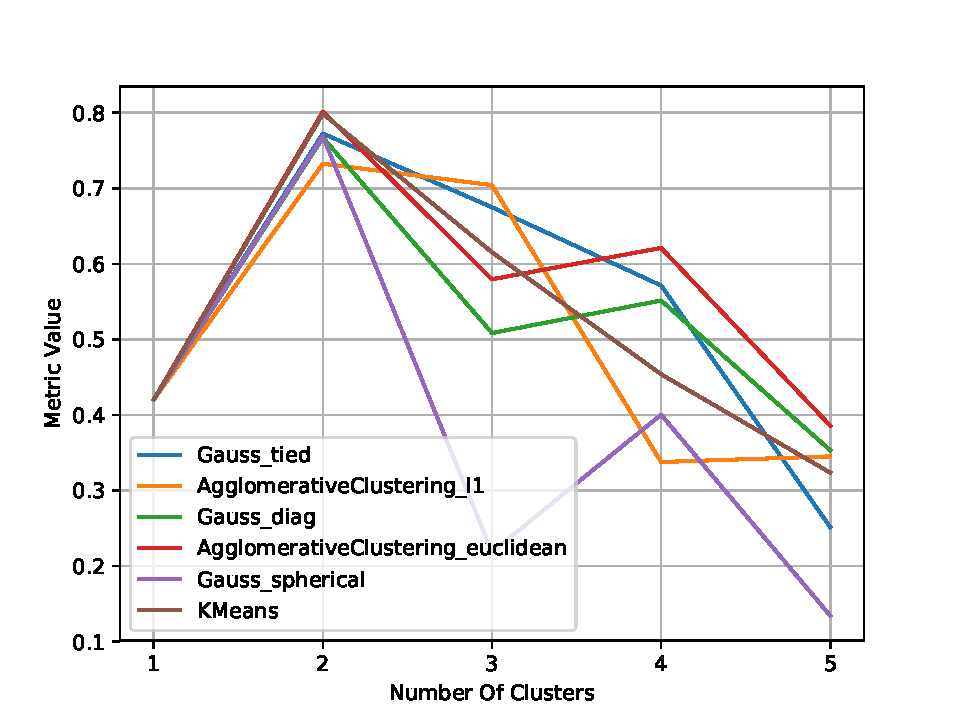
\includegraphics[width=0.7\linewidth]{Images/clusters_number.pdf}

\caption{Результаты подбора оптимального метода и оптимального количества кластеров} \label{choice}
\end{figure}

Мы использовали различные известные алгоритмы кластеризации, при этом мы также варьировали количество кластеров в диапазоне от 1 до 5. Результаты Вы можете видеть на рис.\ref{choice}.



Из результатов данного эксперимента следует, что наилучшим методом кластеризации является KMeans, причем оптимальным количеством кластеров является два.


\section{Кластеризация на два кластера}
\label{sec:cluster}

\begin{figure}[ht!]  

\vspace{-4ex} \centering \subfigure[]{
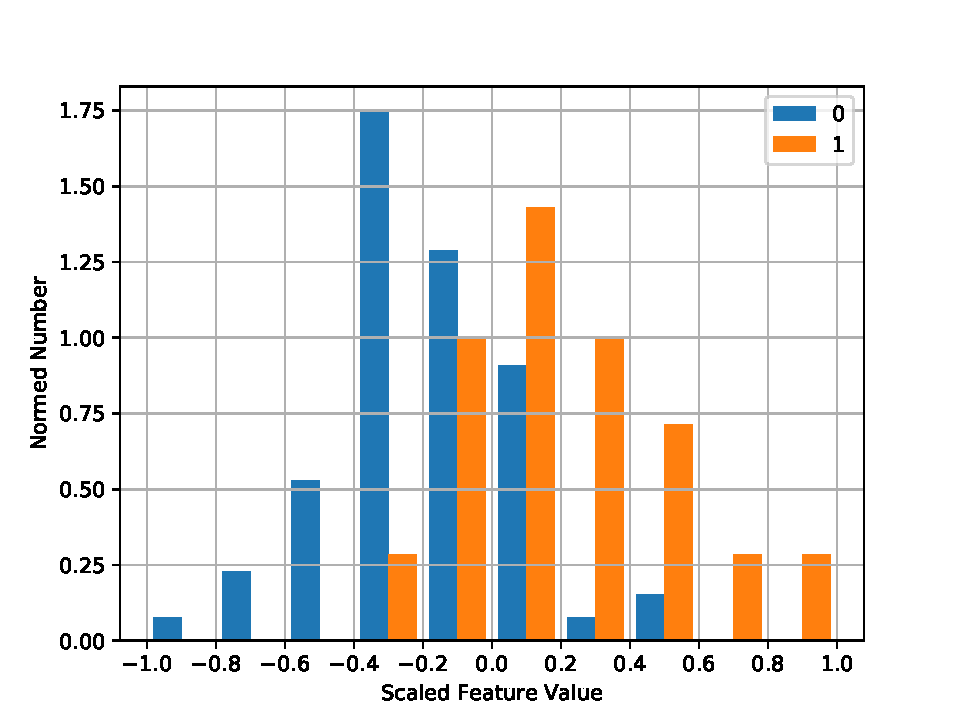
\includegraphics[width=0.3\linewidth]{Images/ManyClusters/17.pdf} \label{1} }  
%\hspace{2ex}
\subfigure[]{
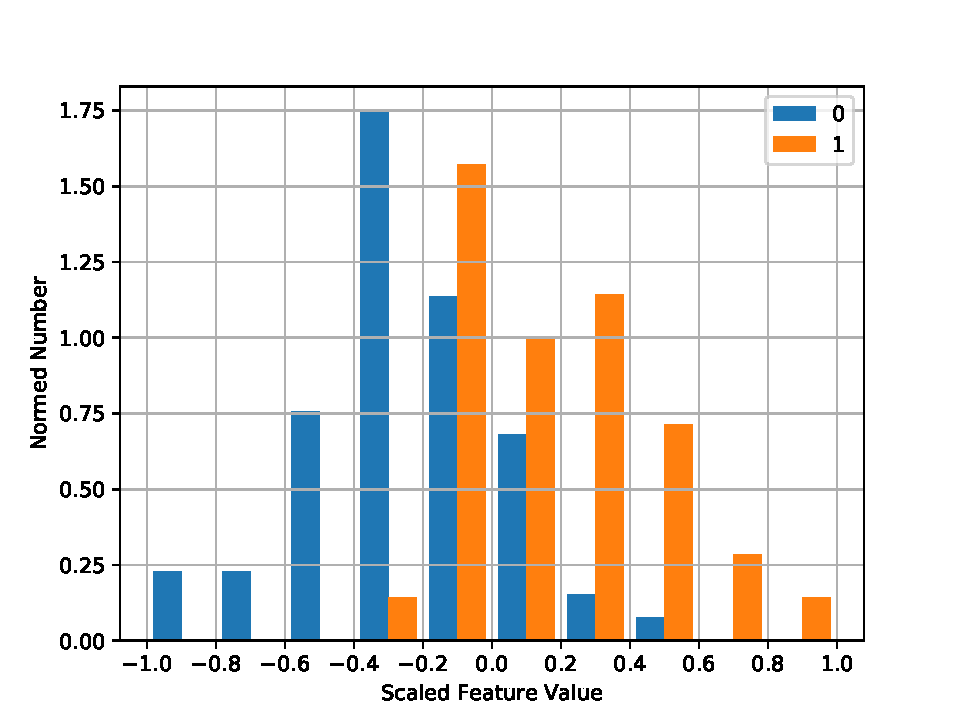
\includegraphics[width=0.3\linewidth]{Images/ManyClusters/16.pdf} \label{2} }  
%\hspace{2ex} 
\centering \subfigure[]{
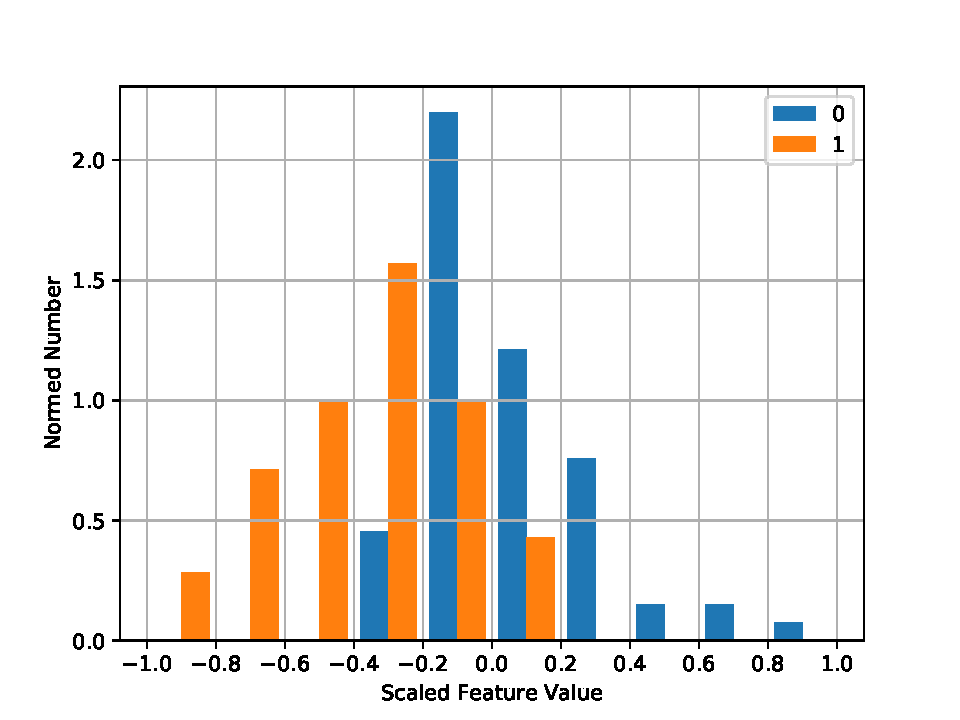
\includegraphics[width=0.3\linewidth]{Images/ManyClusters/15.pdf} \label{3} }  

\vspace{2ex}
\subfigure[]{
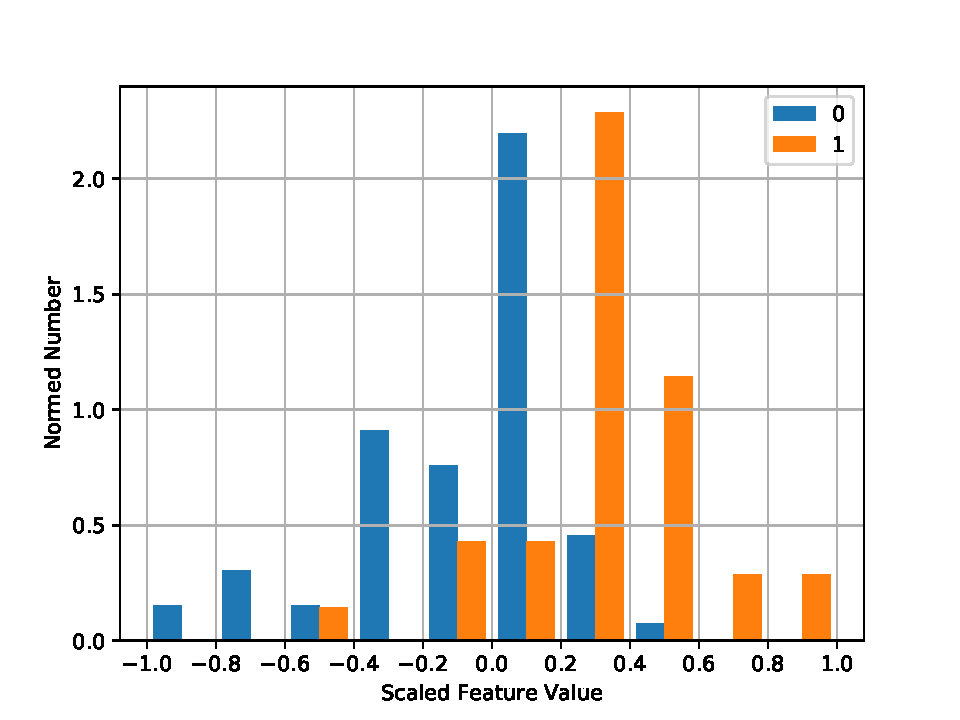
\includegraphics[width=0.3\linewidth]{Images/ManyClusters/14.pdf} \label{4} }  
%\hspace{0.4ex} 
\centering \subfigure[]{
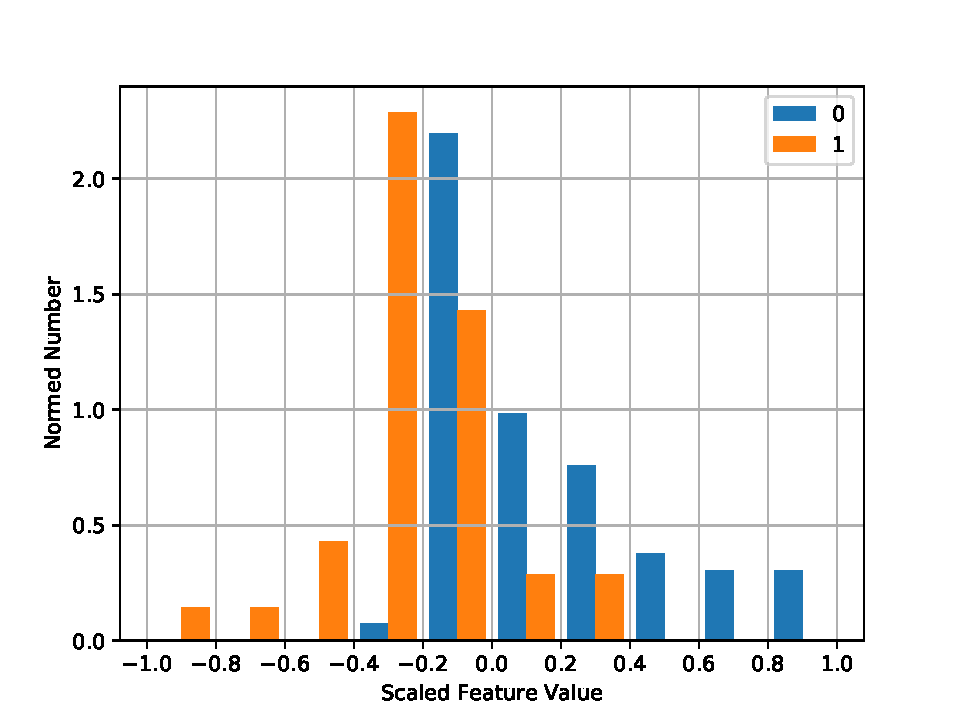
\includegraphics[width=0.3\linewidth]{Images/ManyClusters/13.pdf} \label{5} }  
%\hspace{4ex}
\subfigure[]{
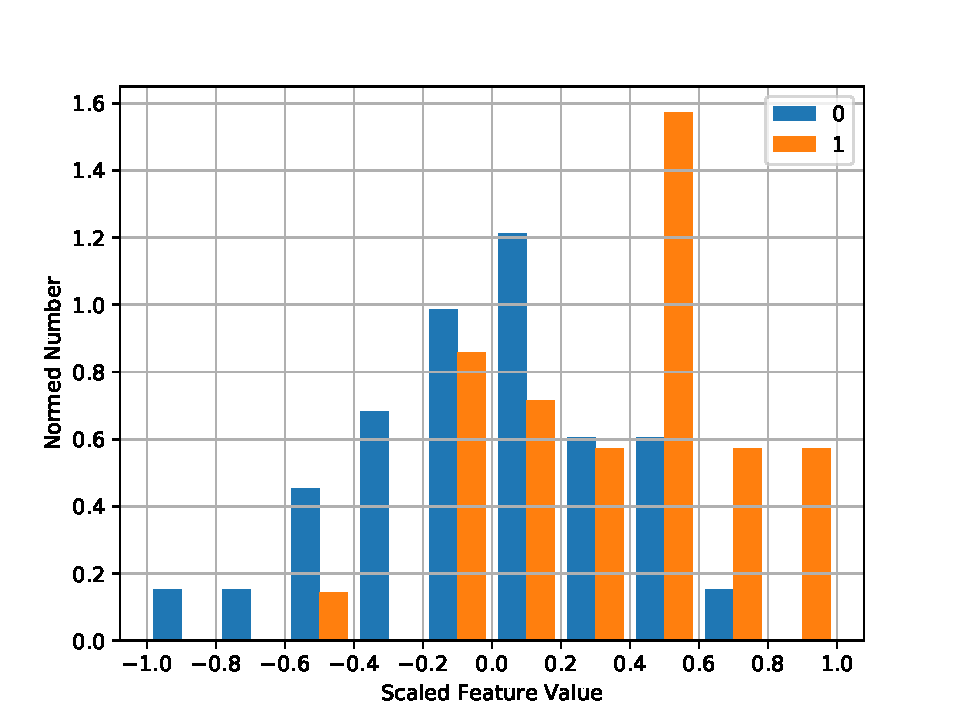
\includegraphics[width=0.3\linewidth]{Images/ManyClusters/12.pdf} \label{6} }  

\vspace{2ex}
\subfigure[]{
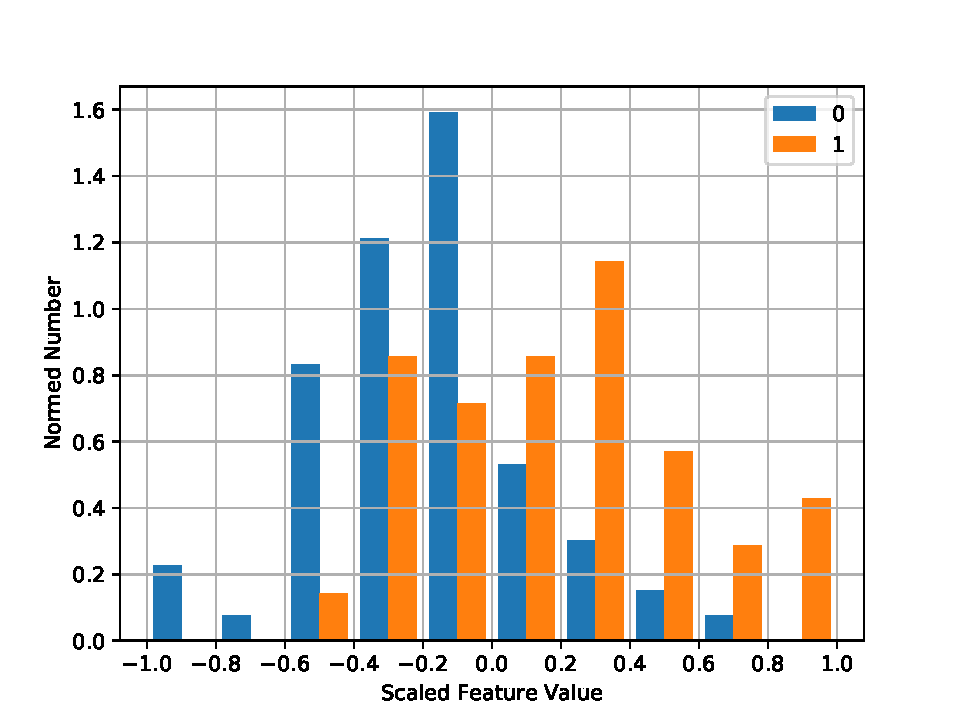
\includegraphics[width=0.3\linewidth]{Images/ManyClusters/11.pdf} \label{7} }  
%\hspace{0.4ex} 
\centering \subfigure[]{
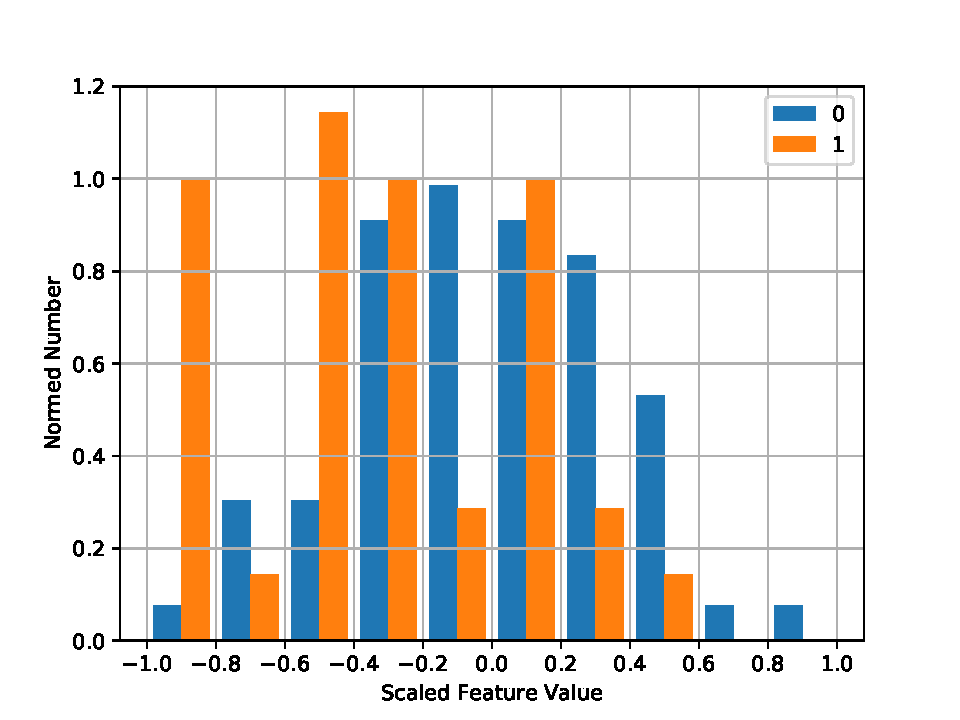
\includegraphics[width=0.3\linewidth]{Images/ManyClusters/10.pdf} \label{8} }  
%\hspace{4ex}
\subfigure[]{
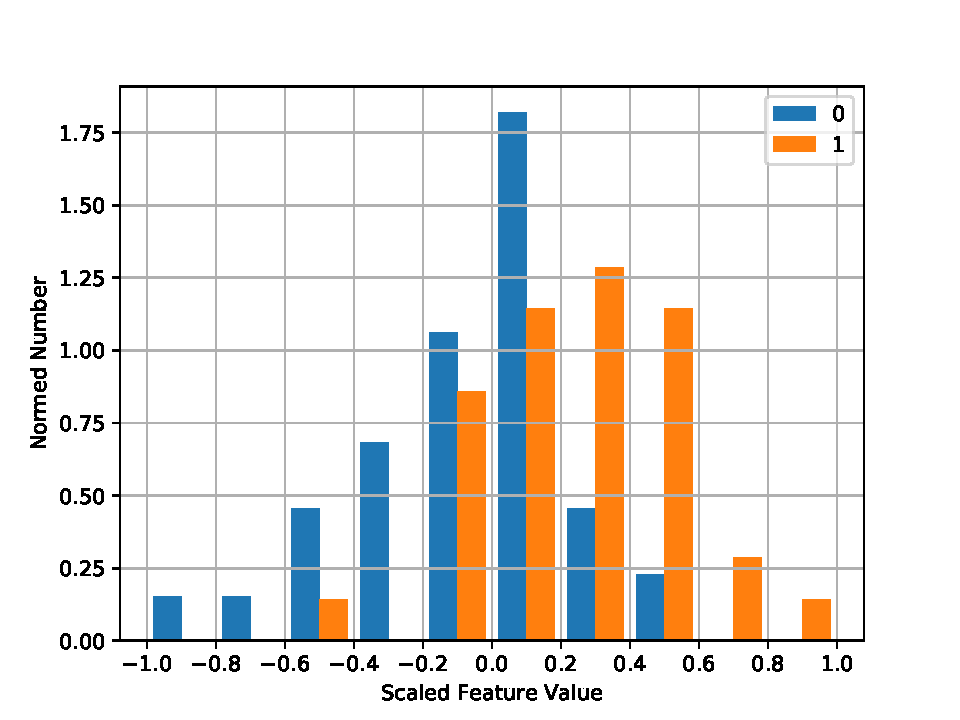
\includegraphics[width=0.3\linewidth]{Images/ManyClusters/9.pdf} \label{9} }  
\vspace{1ex}
\caption{Сравненение распределения для наиболее различающихся признаков (перечислены в порядке возрастания): 
\subref{1} Доля глаголов прошедшего времени, первого лица, единственного числа; 
\subref{2} Доля глаголов 1 лица; 
\subref{3} Часть речи: существительное; 
\subref{4} Часть речи: местоимение-существительное; 
\subref{5} Средняя длина слов (в количестве символов); 
\subref{6} Коэффициент опредмеченности действия (кол. глаголов / кол. существительных); 
\subref{7} Доля местоимений 1 лица ед. числа; 
\subref{8} Сем. роль: предикат; 
\subref{9} Число знаков пунктуации / Число слов.} \label{hist1}
\end{figure}

Выделим наиболее различающиеся признаки у двух кластеров. Мы это сделаем следующим образом: высчитать среднее значение всех признаков для каждого кластера, получить разницу между ними и выбрать топ-9 этих признаков.

Наиболее различающиеся признаки получаются следующие (записаны в порядке убывания):

\begin{itemize}
\item Доля глаголов прошедшего времени, первого лица, единственного числа
\item Доля глаголов 1 лица
\item Часть речи: существительное
\item Часть речи: местоимение-существительное
\item Средняя длина слов (в количестве символов)
\item Коэффициент опредмеченности действия (кол. глаголов / кол. существительных)
\item Доля местоимений 1 лица ед. числа
\item Сем. роль: предикат
\item Число знаков пунктуации / Число слов
\end{itemize}


Посмотрим на распределения значений для соответствующих признаков, причем мы будем смотеть на отмасштабированные значения, т.е. значения, которые получены после первого этапа предобработки. Для каждого признака мы взяли интервал [-1,1], в котором лежат значения этого признака, разбили его на 10 частей, посчитали для каждого кластера количество объектов со значением этого признака в соответствующей части и нормализовали полученные распределения (интеграл по всему интервалу равен единице). Соответствующие гистограммы Вы можете видеть на \ref{hist1}.

\end{document}


